% -*- root: article.tex -*-
Durante o processo de codifica\c{c}\~ao das 18 perguntas sobre boas e m\'as pr\'aticas, 56 categorias emergiram. Classificamos as categorias de acordo com sua recorr\^encia, ou seja, a quantidade de respostas a qual ela foi atribu\'ida. Utilizamos a seguinte escala: baix\'issima recorr\^encia significa menos de 3 respostas, baixa recorr\^encia significa de 3 a 7 respostas, m\'edia recorr\^encia significa de 8 a 20 respostas e alta recorr\^encia significa acima de 20 respostas.

Na Figura \ref{fig:CategoriaXRecorrencia} \'e poss\'ivel observar que o maior conjunto de categorias \'e o de baix\'issima recorr\^encia, ou seja, pouqu\'issimos participantes comentaram sobre esses assuntos. Em seguida, temos o conjunto de m\'edia, baixa e alta recorr\^encia, respectivamente.

\begin{figure}[!htb]
	\centering
	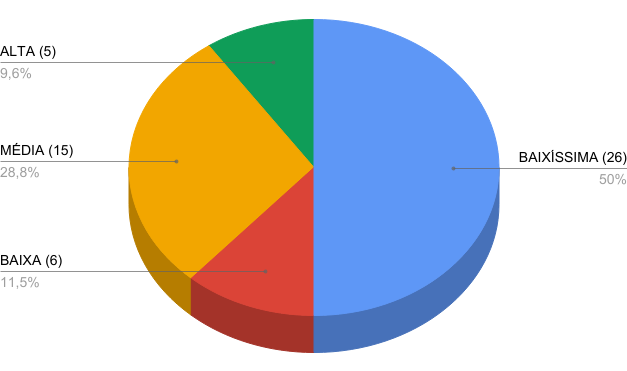
\includegraphics[width=0.45\textwidth]{grafico-recorrencia.png}
	\caption{Distribui\c{c}\~ao das Categorias x Recorr\^encia}
	\label{fig:CategoriaXRecorrencia}
\end{figure}


A Tabela \ref{tab:Categories} apresenta o n\'umero de ocorr\^encias das categorias de alta, m\'edia e baixa recorr\^encia em cada quest\~ao relacionada a boas e m\'as pr\'aticas. A \'ultima linha da tabela, \#Categorias, apresenta quantas categorias emergiram de cada quest\~ao, como cada quest\~ao est\'a diretamente ligada a um elemento do \textit{front-end} Android, podemos interpret\'a-la da seguinte forma: \textbf{quais s\~ao os pontos de aten\c{c}\~ao a serem analisados em determinado elemento Android?} A \'ultima coluna da tabela, \#Q, apresenta em quantas quest\~oes cada categoria surgiu, podemos interpret\'a-la da seguinte forma: \textbf{com base na categoria, quais elementos devem ser investigados}?

% Quando se criam categoriza\c{c}\~oes para auxiliar desenvolvedores a identificar pontos de aten\c{c}\~ao a serem avaliados e onde este pontos devem ser investigados especificamente no c\'odigo, pensando em qualidade de c\'odigo d\'a-se o nome de \textit{smells}. Portanto, nesta se\c{c}\~ao iremos compilar este conjunto de Android \textit{code smells} que identificamos atrav\'es das categoriza\c{c}\~oes.


\begin{table*}[t]
\centering
\footnotesize
\begin{tabular}{@{}p{3.8cm}p{0.3cm}p{.2cm}p{.2cm}p{.2cm}p{.2cm}p{.2cm}p{.2cm}p{.2cm}p{.2cm}p{.2cm}p{.4cm}p{.4cm}p{.4cm}p{.4cm}p{.4cm}p{.4cm}p{.4cm}p{.4cm}p{.4cm}p{0.2cm}@{}}
\toprule
\textbf{Categoria} & \multicolumn{1}{c}{\textbf{\#T}} & Q1 & Q2 & Q3 & Q4 & Q5 & Q6 & Q7 & Q8 & Q9 & Q10 & Q11 & Q12 & Q13 & Q14 & Q15 & Q16 & Q17 & Q18 &  \multicolumn{1}{c}{\textbf{\#Q}} \\
\hline
\multicolumn{2}{c}{\scriptsize{\textbf{ALTA RECORR\^ENCIA}}} \\
L\'ogica em Views							& \multicolumn{1}{c}{53} 	& \multicolumn{1}{c}{12} 	& \multicolumn{1}{c}{15} 	& \multicolumn{1}{c}{6} 	& \multicolumn{1}{c}{8} 	& \multicolumn{1}{c}{3} 	& \multicolumn{1}{c}{8} 	& \multicolumn{1}{c}{--} 	& \multicolumn{1}{c}{1} 	& \multicolumn{1}{c}{--} 	& \multicolumn{1}{c}{--} 	& \multicolumn{1}{c}{--} 	& \multicolumn{1}{c}{--} 	& \multicolumn{1}{c}{--} 	& \multicolumn{1}{c}{--} 	& \multicolumn{1}{c}{--} 	& \multicolumn{1}{c}{--} 	& \multicolumn{1}{c}{--} 	& \multicolumn{1}{c}{--} 	& \multicolumn{1}{c}{7} \\	
Padr\~ao de Nome de Recursos				& \multicolumn{1}{c}{24} 	& \multicolumn{1}{c}{1} 	& \multicolumn{1}{c}{--} 	& \multicolumn{1}{c}{--} 	& \multicolumn{1}{c}{--} 	& \multicolumn{1}{c}{--} 	& \multicolumn{1}{c}{--} 	& \multicolumn{1}{c}{--} 	& \multicolumn{1}{c}{--} 	& \multicolumn{1}{c}{3} 	& \multicolumn{1}{c}{2} 	& \multicolumn{1}{c}{3} 	& \multicolumn{1}{c}{2} 	& \multicolumn{1}{c}{8} 	& \multicolumn{1}{c}{2} 	& \multicolumn{1}{c}{3} 	& \multicolumn{1}{c}{--} 	& \multicolumn{1}{c}{--} 	& \multicolumn{1}{c}{--} 	& \multicolumn{1}{c}{8} \\	
Recursos M\'agicos							& \multicolumn{1}{c}{23} 	& \multicolumn{1}{c}{--} 	& \multicolumn{1}{c}{--} 	& \multicolumn{1}{c}{--} 	& \multicolumn{1}{c}{--} 	& \multicolumn{1}{c}{--} 	& \multicolumn{1}{c}{--} 	& \multicolumn{1}{c}{--} 	& \multicolumn{1}{c}{--} 	& \multicolumn{1}{c}{4} 	& \multicolumn{1}{c}{2} 	& \multicolumn{1}{c}{1} 	& \multicolumn{1}{c}{1} 	& \multicolumn{1}{c}{9} 	& \multicolumn{1}{c}{6} 	& \multicolumn{1}{c}{--} 	& \multicolumn{1}{c}{--} 	& \multicolumn{1}{c}{--} 	& \multicolumn{1}{c}{--} 	& \multicolumn{1}{c}{6} \\	
Views Aninhados								& \multicolumn{1}{c}{21} 	& \multicolumn{1}{c}{--} 	& \multicolumn{1}{c}{--} 	& \multicolumn{1}{c}{--} 	& \multicolumn{1}{c}{--} 	& \multicolumn{1}{c}{1} 	& \multicolumn{1}{c}{--} 	& \multicolumn{1}{c}{--} 	& \multicolumn{1}{c}{--} 	& \multicolumn{1}{c}{9} 	& \multicolumn{1}{c}{9} 	& \multicolumn{1}{c}{--} 	& \multicolumn{1}{c}{--} 	& \multicolumn{1}{c}{--} 	& \multicolumn{1}{c}{--} 	& \multicolumn{1}{c}{--} 	& \multicolumn{1}{c}{--} 	& \multicolumn{1}{c}{1} 	& \multicolumn{1}{c}{1} 	& \multicolumn{1}{c}{5} \\	

\vspace{1sp} \\
\multicolumn{2}{@{}c}{\scriptsize{\textbf{M\'EDIA RECORR\^ENCIA}}} \\ 
Acoplamento Entre Views						& \multicolumn{1}{c}{18} 	& \multicolumn{1}{c}{--} 	& \multicolumn{1}{c}{2} 	& \multicolumn{1}{c}{4} 	& \multicolumn{1}{c}{6} 	& \multicolumn{1}{c}{--} 	& \multicolumn{1}{c}{3} 	& \multicolumn{1}{c}{1} 	& \multicolumn{1}{c}{2} 	& \multicolumn{1}{c}{--} 	& \multicolumn{1}{c}{--} 	& \multicolumn{1}{c}{--} 	& \multicolumn{1}{c}{--} 	& \multicolumn{1}{c}{--} 	& \multicolumn{1}{c}{--} 	& \multicolumn{1}{c}{--} 	& \multicolumn{1}{c}{--} 	& \multicolumn{1}{c}{--} 	& \multicolumn{1}{c}{--} 	& \multicolumn{1}{c}{6} \\
Ciclo de Vida								& \multicolumn{1}{c}{16} 	& \multicolumn{1}{c}{4} 	& \multicolumn{1}{c}{3} 	& \multicolumn{1}{c}{3} 	& \multicolumn{1}{c}{5} 	& \multicolumn{1}{c}{--} 	& \multicolumn{1}{c}{--} 	& \multicolumn{1}{c}{1} 	& \multicolumn{1}{c}{--} 	& \multicolumn{1}{c}{--} 	& \multicolumn{1}{c}{--} 	& \multicolumn{1}{c}{--} 	& \multicolumn{1}{c}{--} 	& \multicolumn{1}{c}{--} 	& \multicolumn{1}{c}{--} 	& \multicolumn{1}{c}{--} 	& \multicolumn{1}{c}{--} 	& \multicolumn{1}{c}{--} 	& \multicolumn{1}{c}{--} 	& \multicolumn{1}{c}{5} \\
Use Include									& \multicolumn{1}{c}{15} 	& \multicolumn{1}{c}{--} 	& \multicolumn{1}{c}{--} 	& \multicolumn{1}{c}{--} 	& \multicolumn{1}{c}{--} 	& \multicolumn{1}{c}{--} 	& \multicolumn{1}{c}{--} 	& \multicolumn{1}{c}{--} 	& \multicolumn{1}{c}{--} 	& \multicolumn{1}{c}{12} 	& \multicolumn{1}{c}{2} 	& \multicolumn{1}{c}{--} 	& \multicolumn{1}{c}{--} 	& \multicolumn{1}{c}{--} 	& \multicolumn{1}{c}{--} 	& \multicolumn{1}{c}{--} 	& \multicolumn{1}{c}{--} 	& \multicolumn{1}{c}{1} 	& \multicolumn{1}{c}{--} 	& \multicolumn{1}{c}{3} \\
Padr\~ao View Holder						& \multicolumn{1}{c}{14} 	& \multicolumn{1}{c}{--} 	& \multicolumn{1}{c}{--} 	& \multicolumn{1}{c}{--} 	& \multicolumn{1}{c}{--} 	& \multicolumn{1}{c}{12} 	& \multicolumn{1}{c}{2} 	& \multicolumn{1}{c}{--} 	& \multicolumn{1}{c}{--} 	& \multicolumn{1}{c}{--} 	& \multicolumn{1}{c}{--} 	& \multicolumn{1}{c}{--} 	& \multicolumn{1}{c}{--} 	& \multicolumn{1}{c}{--} 	& \multicolumn{1}{c}{--} 	& \multicolumn{1}{c}{--} 	& \multicolumn{1}{c}{--} 	& \multicolumn{1}{c}{--} 	& \multicolumn{1}{c}{--} 	& \multicolumn{1}{c}{2} \\
Tamanho de Imagens Importam					& \multicolumn{1}{c}{12} 	& \multicolumn{1}{c}{--} 	& \multicolumn{1}{c}{--} 	& \multicolumn{1}{c}{--} 	& \multicolumn{1}{c}{--} 	& \multicolumn{1}{c}{--} 	& \multicolumn{1}{c}{--} 	& \multicolumn{1}{c}{--} 	& \multicolumn{1}{c}{--} 	& \multicolumn{1}{c}{1} 	& \multicolumn{1}{c}{1} 	& \multicolumn{1}{c}{--} 	& \multicolumn{1}{c}{--} 	& \multicolumn{1}{c}{--} 	& \multicolumn{1}{c}{--} 	& \multicolumn{1}{c}{4} 	& \multicolumn{1}{c}{6} 	& \multicolumn{1}{c}{--} 	& \multicolumn{1}{c}{--} 	& \multicolumn{1}{c}{4} \\
Comportamento Suspeito						& \multicolumn{1}{c}{14} 	& \multicolumn{1}{c}{1} 	& \multicolumn{1}{c}{1} 	& \multicolumn{1}{c}{--} 	& \multicolumn{1}{c}{--} 	& \multicolumn{1}{c}{1} 	& \multicolumn{1}{c}{3} 	& \multicolumn{1}{c}{5} 	& \multicolumn{1}{c}{3} 	& \multicolumn{1}{c}{--} 	& \multicolumn{1}{c}{--} 	& \multicolumn{1}{c}{--} 	& \multicolumn{1}{c}{--} 	& \multicolumn{1}{c}{--} 	& \multicolumn{1}{c}{--} 	& \multicolumn{1}{c}{--} 	& \multicolumn{1}{c}{--} 	& \multicolumn{1}{c}{--} 	& \multicolumn{1}{c}{--} 	& \multicolumn{1}{c}{6} \\
Classe Deus/Longa*							& \multicolumn{1}{c}{11} 	& \multicolumn{1}{c}{1} 	& \multicolumn{1}{c}{4} 	& \multicolumn{1}{c}{1} 	& \multicolumn{1}{c}{2} 	& \multicolumn{1}{c}{--} 	& \multicolumn{1}{c}{1} 	& \multicolumn{1}{c}{--} 	& \multicolumn{1}{c}{1} 	& \multicolumn{1}{c}{--} 	& \multicolumn{1}{c}{--} 	& \multicolumn{1}{c}{--} 	& \multicolumn{1}{c}{1} 	& \multicolumn{1}{c}{--} 	& \multicolumn{1}{c}{--} 	& \multicolumn{1}{c}{--} 	& \multicolumn{1}{c}{--} 	& \multicolumn{1}{c}{--} 	& \multicolumn{1}{c}{--} 	& \multicolumn{1}{c}{7} \\
Use Fragment								& \multicolumn{1}{c}{11} 	& \multicolumn{1}{c}{3} 	& \multicolumn{1}{c}{2} 	& \multicolumn{1}{c}{5} 	& \multicolumn{1}{c}{1} 	& \multicolumn{1}{c}{--} 	& \multicolumn{1}{c}{--} 	& \multicolumn{1}{c}{--} 	& \multicolumn{1}{c}{--} 	& \multicolumn{1}{c}{--} 	& \multicolumn{1}{c}{--} 	& \multicolumn{1}{c}{--} 	& \multicolumn{1}{c}{--} 	& \multicolumn{1}{c}{--} 	& \multicolumn{1}{c}{--} 	& \multicolumn{1}{c}{--} 	& \multicolumn{1}{c}{--} 	& \multicolumn{1}{c}{--} 	& \multicolumn{1}{c}{--} 	& \multicolumn{1}{c}{4} \\
Use Imagens Vetoriais						& \multicolumn{1}{c}{11} 	& \multicolumn{1}{c}{--} 	& \multicolumn{1}{c}{--} 	& \multicolumn{1}{c}{--} 	& \multicolumn{1}{c}{--} 	& \multicolumn{1}{c}{--} 	& \multicolumn{1}{c}{--} 	& \multicolumn{1}{c}{--} 	& \multicolumn{1}{c}{--} 	& \multicolumn{1}{c}{--} 	& \multicolumn{1}{c}{--} 	& \multicolumn{1}{c}{--} 	& \multicolumn{1}{c}{--} 	& \multicolumn{1}{c}{--} 	& \multicolumn{1}{c}{--} 	& \multicolumn{1}{c}{11} 	& \multicolumn{1}{c}{--} 	& \multicolumn{1}{c}{--} 	& \multicolumn{1}{c}{--} 	& \multicolumn{1}{c}{1} \\
Fragment Apenas Se Necess\'ario				& \multicolumn{1}{c}{10} 	& \multicolumn{1}{c}{--} 	& \multicolumn{1}{c}{--} 	& \multicolumn{1}{c}{8} 	& \multicolumn{1}{c}{2} 	& \multicolumn{1}{c}{--} 	& \multicolumn{1}{c}{--} 	& \multicolumn{1}{c}{--} 	& \multicolumn{1}{c}{--} 	& \multicolumn{1}{c}{--} 	& \multicolumn{1}{c}{--} 	& \multicolumn{1}{c}{--} 	& \multicolumn{1}{c}{--} 	& \multicolumn{1}{c}{--} 	& \multicolumn{1}{c}{--} 	& \multicolumn{1}{c}{--} 	& \multicolumn{1}{c}{--} 	& \multicolumn{1}{c}{--} 	& \multicolumn{1}{c}{--} 	& \multicolumn{1}{c}{2} \\
Use Arquiteturas Conhecidas					& \multicolumn{1}{c}{9} 	& \multicolumn{1}{c}{--} 	& \multicolumn{1}{c}{--} 	& \multicolumn{1}{c}{1} 	& \multicolumn{1}{c}{--} 	& \multicolumn{1}{c}{2} 	& \multicolumn{1}{c}{--} 	& \multicolumn{1}{c}{--} 	& \multicolumn{1}{c}{--} 	& \multicolumn{1}{c}{--} 	& \multicolumn{1}{c}{--} 	& \multicolumn{1}{c}{--} 	& \multicolumn{1}{c}{--} 	& \multicolumn{1}{c}{--} 	& \multicolumn{1}{c}{--} 	& \multicolumn{1}{c}{--} 	& \multicolumn{1}{c}{--} 	& \multicolumn{1}{c}{5} 	& \multicolumn{1}{c}{1} 	& \multicolumn{1}{c}{4} \\
Recurso de Estilo Deus						& \multicolumn{1}{c}{8} 	& \multicolumn{1}{c}{--} 	& \multicolumn{1}{c}{--} 	& \multicolumn{1}{c}{--} 	& \multicolumn{1}{c}{--} 	& \multicolumn{1}{c}{--} 	& \multicolumn{1}{c}{--} 	& \multicolumn{1}{c}{--} 	& \multicolumn{1}{c}{--} 	& \multicolumn{1}{c}{--} 	& \multicolumn{1}{c}{--} 	& \multicolumn{1}{c}{5} 	& \multicolumn{1}{c}{3} 	& \multicolumn{1}{c}{--} 	& \multicolumn{1}{c}{--} 	& \multicolumn{1}{c}{--} 	& \multicolumn{1}{c}{--} 	& \multicolumn{1}{c}{--} 	& \multicolumn{1}{c}{--} 	& \multicolumn{1}{c}{2} \\
Recurso de Strings Bagun\c{c}ado			& \multicolumn{1}{c}{8} 	& \multicolumn{1}{c}{--} 	& \multicolumn{1}{c}{--} 	& \multicolumn{1}{c}{--} 	& \multicolumn{1}{c}{--} 	& \multicolumn{1}{c}{--} 	& \multicolumn{1}{c}{--} 	& \multicolumn{1}{c}{--} 	& \multicolumn{1}{c}{--} 	& \multicolumn{1}{c}{--} 	& \multicolumn{1}{c}{--} 	& \multicolumn{1}{c}{--} 	& \multicolumn{1}{c}{--} 	& \multicolumn{1}{c}{4} 	& \multicolumn{1}{c}{4} 	& \multicolumn{1}{c}{--} 	& \multicolumn{1}{c}{--} 	& \multicolumn{1}{c}{--} 	& \multicolumn{1}{c}{--} 	& \multicolumn{1}{c}{2} \\
Atributos de Estilos Repetidos				& \multicolumn{1}{c}{8} 	& \multicolumn{1}{c}{--} 	& \multicolumn{1}{c}{--} 	& \multicolumn{1}{c}{--} 	& \multicolumn{1}{c}{--} 	& \multicolumn{1}{c}{--} 	& \multicolumn{1}{c}{--} 	& \multicolumn{1}{c}{--} 	& \multicolumn{1}{c}{--} 	& \multicolumn{1}{c}{1} 	& \multicolumn{1}{c}{2} 	& \multicolumn{1}{c}{2} 	& \multicolumn{1}{c}{2} 	& \multicolumn{1}{c}{--} 	& \multicolumn{1}{c}{--} 	& \multicolumn{1}{c}{--} 	& \multicolumn{1}{c}{--} 	& \multicolumn{1}{c}{1} 	& \multicolumn{1}{c}{--} 	& \multicolumn{1}{c}{5} \\

\vspace*{1sp} \\
\multicolumn{2}{@{}c}{\scriptsize{\textbf{BAIXA RECORR\^ENCIA}}} \\
Activity Inexistente  						& \multicolumn{1}{c}{7} 	& \multicolumn{1}{c}{2} 	& \multicolumn{1}{c}{4} 	& \multicolumn{1}{c}{--} 	& \multicolumn{1}{c}{--} 	& \multicolumn{1}{c}{--} 	& \multicolumn{1}{c}{--} 	& \multicolumn{1}{c}{--} 	& \multicolumn{1}{c}{1} 	& \multicolumn{1}{c}{--} 	& \multicolumn{1}{c}{--} 	& \multicolumn{1}{c}{--} 	& \multicolumn{1}{c}{--} 	& \multicolumn{1}{c}{--} 	& \multicolumn{1}{c}{--} 	& \multicolumn{1}{c}{--} 	& \multicolumn{1}{c}{--} 	& \multicolumn{1}{c}{--} 	& \multicolumn{1}{c}{--} 	& \multicolumn{1}{c}{3} \\
Evite Imagens								& \multicolumn{1}{c}{7} 	& \multicolumn{1}{c}{--} 	& \multicolumn{1}{c}{--} 	& \multicolumn{1}{c}{--} 	& \multicolumn{1}{c}{--} 	& \multicolumn{1}{c}{--} 	& \multicolumn{1}{c}{--} 	& \multicolumn{1}{c}{--} 	& \multicolumn{1}{c}{--} 	& \multicolumn{1}{c}{1} 	& \multicolumn{1}{c}{--} 	& \multicolumn{1}{c}{--} 	& \multicolumn{1}{c}{--} 	& \multicolumn{1}{c}{--} 	& \multicolumn{1}{c}{--} 	& \multicolumn{1}{c}{4} 	& \multicolumn{1}{c}{2} 	& \multicolumn{1}{c}{--} 	& \multicolumn{1}{c}{--} 	& \multicolumn{1}{c}{3} \\
Reuso Excessivo de Strings					& \multicolumn{1}{c}{6} 	& \multicolumn{1}{c}{--} 	& \multicolumn{1}{c}{--} 	& \multicolumn{1}{c}{--} 	& \multicolumn{1}{c}{--} 	& \multicolumn{1}{c}{--} 	& \multicolumn{1}{c}{--} 	& \multicolumn{1}{c}{--} 	& \multicolumn{1}{c}{--} 	& \multicolumn{1}{c}{--} 	& \multicolumn{1}{c}{--} 	& \multicolumn{1}{c}{--} 	& \multicolumn{1}{c}{--} 	& \multicolumn{1}{c}{2} 	& \multicolumn{1}{c}{4} 	& \multicolumn{1}{c}{--} 	& \multicolumn{1}{c}{--} 	& \multicolumn{1}{c}{--} 	& \multicolumn{1}{c}{--} 	& \multicolumn{1}{c}{2} \\
Adapter Flex\'ivel							& \multicolumn{1}{c}{6} 	& \multicolumn{1}{c}{--} 	& \multicolumn{1}{c}{--} 	& \multicolumn{1}{c}{--} 	& \multicolumn{1}{c}{--} 	& \multicolumn{1}{c}{3} 	& \multicolumn{1}{c}{2} 	& \multicolumn{1}{c}{--} 	& \multicolumn{1}{c}{--} 	& \multicolumn{1}{c}{--} 	& \multicolumn{1}{c}{1} 	& \multicolumn{1}{c}{--} 	& \multicolumn{1}{c}{--} 	& \multicolumn{1}{c}{--} 	& \multicolumn{1}{c}{--} 	& \multicolumn{1}{c}{--} 	& \multicolumn{1}{c}{--} 	& \multicolumn{1}{c}{--} 	& \multicolumn{1}{c}{--} 	& \multicolumn{1}{c}{3} \\
Heran\c{c}a**								& \multicolumn{1}{c}{5} 	& \multicolumn{1}{c}{2} 	& \multicolumn{1}{c}{--} 	& \multicolumn{1}{c}{2} 	& \multicolumn{1}{c}{--} 	& \multicolumn{1}{c}{1} 	& \multicolumn{1}{c}{--} 	& \multicolumn{1}{c}{--} 	& \multicolumn{1}{c}{--} 	& \multicolumn{1}{c}{--} 	& \multicolumn{1}{c}{--} 	& \multicolumn{1}{c}{--} 	& \multicolumn{1}{c}{--} 	& \multicolumn{1}{c}{--} 	& \multicolumn{1}{c}{--} 	& \multicolumn{1}{c}{--} 	& \multicolumn{1}{c}{--} 	& \multicolumn{1}{c}{--} 	& \multicolumn{1}{c}{--} 	& \multicolumn{1}{c}{3} \\
Listener Escondido							& \multicolumn{1}{c}{3} 	& \multicolumn{1}{c}{--} 	& \multicolumn{1}{c}{--} 	& \multicolumn{1}{c}{--} 	& \multicolumn{1}{c}{--} 	& \multicolumn{1}{c}{--} 	& \multicolumn{1}{c}{--} 	& \multicolumn{1}{c}{--} 	& \multicolumn{1}{c}{3} 	& \multicolumn{1}{c}{--} 	& \multicolumn{1}{c}{--} 	& \multicolumn{1}{c}{--} 	& \multicolumn{1}{c}{--} 	& \multicolumn{1}{c}{--} 	& \multicolumn{1}{c}{--} 	& \multicolumn{1}{c}{--} 	& \multicolumn{1}{c}{--} 	& \multicolumn{1}{c}{--} 	& \multicolumn{1}{c}{--} 	& \multicolumn{1}{c}{1} \\
Opera\c{c}\~oes de IO							& \multicolumn{1}{c}{6} 	& \multicolumn{1}{c}{--} 	& \multicolumn{1}{c}{3} 	& \multicolumn{1}{c}{--} 	& \multicolumn{1}{c}{2} 	& \multicolumn{1}{c}{--} 	& \multicolumn{1}{c}{1} 	& \multicolumn{1}{c}{--} 	& \multicolumn{1}{c}{--} 	& \multicolumn{1}{c}{--} 	& \multicolumn{1}{c}{--} 	& \multicolumn{1}{c}{--} 	& \multicolumn{1}{c}{--} 	& \multicolumn{1}{c}{--} 	& \multicolumn{1}{c}{--} 	& \multicolumn{1}{c}{--} 	& \multicolumn{1}{c}{--} 	& \multicolumn{1}{c}{--} 	& \multicolumn{1}{c}{--} 	& \multicolumn{1}{c}{3} \\
\hline
\multicolumn{2}{r}{\textbf{\#Totais}}		& \multicolumn{1}{c}{35} 	& \multicolumn{1}{c}{37} 	& \multicolumn{1}{c}{35} 	& \multicolumn{1}{c}{26} 	& \multicolumn{1}{c}{23} 	& \multicolumn{1}{c}{20} 	& \multicolumn{1}{c}{11} 	& \multicolumn{1}{c}{11} 	& \multicolumn{1}{c}{31} 	& \multicolumn{1}{c}{19} 	& \multicolumn{1}{c}{11} 	& \multicolumn{1}{c}{9} 	& \multicolumn{1}{c}{23} 	& \multicolumn{1}{c}{16} 	& \multicolumn{1}{c}{22} 	& \multicolumn{1}{c}{8} 	& \multicolumn{1}{c}{11} 	& \multicolumn{1}{c}{2} \\
\hline
\multicolumn{2}{r}{\textbf{\#Categorias}}	& \multicolumn{1}{c}{10} 	& \multicolumn{1}{c}{10} 	& \multicolumn{1}{c}{9} 	& \multicolumn{1}{c}{7} 	& \multicolumn{1}{c}{7} 	& \multicolumn{1}{c}{7} 	& \multicolumn{1}{c}{4} 	& \multicolumn{1}{c}{6} 	& \multicolumn{1}{c}{7} 	& \multicolumn{1}{c}{7} 	& \multicolumn{1}{c}{4} 	& \multicolumn{1}{c}{5} 	& \multicolumn{1}{c}{4} 	& \multicolumn{1}{c}{4} 	& \multicolumn{1}{c}{4} 	& \multicolumn{1}{c}{2} 	& \multicolumn{1}{c}{6} 	& \multicolumn{1}{c}{2} \\
\hline
% \multicolumn{20}{@{}l@{}}{* Classe Deus \cite{Riel} e Classe Longa \cite{RefactoringFowler1999} s\~ao \textit{code smells} tradicionais previamente definidos em literaturas. ** Heran\c{c}a \'e um conceito da Programa\c{c}\~ao Orientada a Objetos \cite{WikipediaInhiritance}. \textbf{\#T}: recorr\^encia geral da categoria. \textbf{\#Q}: total de quest\~oes distintas em cada categoria. A linha \textbf{\#Totais}: total de respostas obtidas em cada quest\~ao. \textbf{\#Categorias}: total de categorias distinstas de cada quest\~ao.} \\

\multicolumn{20}{@{}l}{* Classe Deus \cite{Riel} e Classe Longa \cite{RefactoringFowler1999} s\~ao cheiros de c\'odigo tradicionais previamente definidos em literaturas.} \\
\multicolumn{20}{@{}l}{** Heran\c{c}a \'e um conceito da Programa\c{c}\~ao Orientada a Objetos \cite{WikipediaInhiritance}.} \\
\multicolumn{20}{@{}l}{Coluna \textbf{\#T}: recorr\^encia geral da categoria.} \\
\multicolumn{20}{@{}l}{Coluna \textbf{\#Q}: total de quest\~oes distintas em cada categoria.} \\
\multicolumn{20}{@{}l}{Linha \textbf{\#Totais}: total de respostas obtidas em cada quest\~ao.} \\
\multicolumn{20}{@{}l}{Linha \textbf{\#Categorias}: total de categorias distinstas de cada quest\~ao.} \\
\toprule
\end{tabular}
\caption{Lista de categorias de alta, m\'edia e baixa recorr\^encia.}
\label{tab:Categories}
\end{table*}


Esta se\c{c}\~ao est\'a organizada em 4 subse\c{c}\~oes, respectivamente abordando sobre as categorias de alta, m\'edia, baixa e baix\'issima recorr\^encia. A quantidade de respostas recebida por cada categoria \'e apresentada em detalhes na Tabela \ref{tab:Categories}.

\subsection{Categorias de Alta Recorr\^encia}
Obtivemos 4 categorias consideradas de alta recorr\^encia: L\'ogica em Views, Padr\~ao de Nome de Recursos, Recursos M\'agicos e Views Aninhados.


% \begin{table*}[t]
% \centering
% \caption{Lista de categorias de alta recorr\^encia.}
% \footnotesize
% \begin{tabular}{@{}p{2.9cm}p{1cm}|p{0.3cm}p{0.3cm}p{0.3cm}p{0.3cm}p{0.3cm}p{0.3cm}p{0.3cm}p{0.3cm}p{0.4cm}p{0.4cm}p{0.4cm}p{0.4cm}p{0.4cm}p{0.4cm}p{0.4cm}p{0.4cm}|p{1.5cm}@{}}
% \toprule
% \textbf{Categoria}	& \textbf{\#Total} 	& Q1 	& Q2 	& Q3 	& Q4 	& Q5 	& Q6 	& Q8 	& Q9 	& Q10 	& Q11 	& Q12 	& Q13 	& Q14 	& Q15 	& Q17 	& Q18 	&  \textbf{\#Quest\~oes} \\
% \hline
% No Logic In View				& 	\multicolumn{1}{c|}{53} 	& \multicolumn{1}{c}{12} 	& \multicolumn{1}{c}{15} 	& \multicolumn{1}{c}{6} 	& \multicolumn{1}{c}{8} 	& \multicolumn{1}{c}{3} 	& \multicolumn{1}{c}{8} 	& \multicolumn{1}{c}{1} 	& \multicolumn{1}{c}{--} 	& \multicolumn{1}{c}{--} 	& \multicolumn{1}{c}{--} 	& \multicolumn{1}{c}{--} 	& \multicolumn{1}{c}{--} 	& \multicolumn{1}{c}{--} 	& \multicolumn{1}{c}{--} 	& \multicolumn{1}{c}{--} 	& \multicolumn{1}{c|}{0} 	& \multicolumn{1}{c}{7}	\\
% Resource Name Pattern			& 	\multicolumn{1}{c|}{24} 	& \multicolumn{1}{c}{1} 	& \multicolumn{1}{c}{--} 	& \multicolumn{1}{c}{--} 	& \multicolumn{1}{c}{--} 	& \multicolumn{1}{c}{--} 	& \multicolumn{1}{c}{--} 	& \multicolumn{1}{c}{--} 	& \multicolumn{1}{c}{3} 	& \multicolumn{1}{c}{2} 	& \multicolumn{1}{c}{3} 	& \multicolumn{1}{c}{2} 	& \multicolumn{1}{c}{8} 	& \multicolumn{1}{c}{2} 	& \multicolumn{1}{c}{3} 	& \multicolumn{1}{c}{--} 	& \multicolumn{1}{c|}{0} 	& \multicolumn{1}{c}{8}	\\
% Magic Resource					& 	\multicolumn{1}{c|}{23} 	& \multicolumn{1}{c}{--} 	& \multicolumn{1}{c}{--} 	& \multicolumn{1}{c}{--} 	& \multicolumn{1}{c}{--} 	& \multicolumn{1}{c}{--} 	& \multicolumn{1}{c}{--} 	& \multicolumn{1}{c}{--} 	& \multicolumn{1}{c}{4} 	& \multicolumn{1}{c}{2} 	& \multicolumn{1}{c}{1} 	& \multicolumn{1}{c}{1} 	& \multicolumn{1}{c}{9} 	& \multicolumn{1}{c}{6} 	& \multicolumn{1}{c}{--} 	& \multicolumn{1}{c}{--} 	& \multicolumn{1}{c|}{0} 	& \multicolumn{1}{c}{6}	\\
% Nested Layout					& 	\multicolumn{1}{c|}{21} 	& \multicolumn{1}{c}{--} 	& \multicolumn{1}{c}{--} 	& \multicolumn{1}{c}{--} 	& \multicolumn{1}{c}{--} 	& \multicolumn{1}{c}{1} 	& \multicolumn{1}{c}{--} 	& \multicolumn{1}{c}{--} 	& \multicolumn{1}{c}{9} 	& \multicolumn{1}{c}{9} 	& \multicolumn{1}{c}{--} 	& \multicolumn{1}{c}{--} 	& \multicolumn{1}{c}{--} 	& \multicolumn{1}{c}{--} 	& \multicolumn{1}{c}{--} 	& \multicolumn{1}{c}{1} 	& \multicolumn{1}{c|}{1} 	& \multicolumn{1}{c}{5}	\\
% % \hline
% % \multicolumn{2}{r}{\textbf{\#Total}}										& \multicolumn{1}{c}{13} 	& \multicolumn{1}{c}{15} 	& \multicolumn{1}{c}{6} 	& \multicolumn{1}{c}{8} 	& \multicolumn{1}{c}{4} 	& \multicolumn{1}{c}{8} 	& \multicolumn{1}{c}{1} 	& \multicolumn{1}{c}{16} 	& \multicolumn{1}{c}{13} 	& \multicolumn{1}{c}{4} 	& \multicolumn{1}{c}{3} 	& \multicolumn{1}{c}{17} 	& \multicolumn{1}{c}{8} 	& \multicolumn{1}{c}{3} 	& \multicolumn{1}{c}{1} 	& \multicolumn{1}{c}{1} 	& \\
% \hline
% \multicolumn{19}{@{}l}{\scriptsize{* As categorias de alta recorr\^encia n\~ao n\~ao receberam respostas \`as quest\~oes Q7 e Q16.}} \\
% \toprule
% \end{tabular}
% \label{tab:CategoriasAltaRecorrencia}
% \end{table*}

\subsubsection{L\'ogica em Views}
Esta categoria re\'une respostas que indicam como m\'a pr\'atica haver regras de neg\'ocio nos elementos \textsc{Activitys}, \textsc{Fragments}, \textsc{Listeners} e \textsc{Adapters}. De forma similar, respostas indicam como boas pr\'aticas que esses elementos apenas contenham c\'odigos relacionados a interface com o usu\'ario, e para isso sugerem o uso de alguns padr\~oes, foram eles: MVP (\textit{Model-View-Presenter}) \cite{MartinFowlerGUIArchitectures, WikipediaMVP}, MVVM (\textit{Model-View-ViewModel}) \cite{WikipediaMVVM} e \textit{Clean Architecture} \cite{CleanArchitecture}. Exemplos de frases que indicaram m\'as pr\'aticas s\~ao: P16 sobre \textsc{Activitys} diz \textit{``Fazer l\'ogica de neg\'ocio''} (tradu\c{c}\~ao livre), P19 diz \textit{``Colocar regra de neg\'ocio no adapter''} e P11 diz \textit{``Manter l\'ogica de neg\'ocio em Fragments''} (tradu\c{c}\~ao livre). Exemplos de frases que indicaram boas pr\'atica s\~ao: P16 diz sobre \textsc{Activitys} \textit{``Elas representam uma \'unica tela e apenas interagem com a UI, qualquer l\'ogica deve ser delegada para outra classe''} (tradu\c{c}\~ao livre), P23 diz \textit{``Apenas c\'odigo relacionado \`a Interface de Usu\'ario nas Activities''}, P40 diz \textit{``Adapters devem apenas se preocupar sobre como mostrar os dados, sem trabalh\'a-los''}, P2 diz \textit{``As activitys que eu crio normalmente tem um prop\'osito \'unico e estado b\'asico [...] eu uso MVP a maior parte do tempo, ent\~ao minhas activitys normalmente representam uma view no MVP''}. Os elementos afetados por essa categoria s\~ao: \textsc{Activitys}, \textsc{Fragments}, \textsc{Listeners} e \textsc{Adapters}. 

\subsubsection{Padr\~ao de Nome de Recursos}
Esta categoria re\'une respostas que indicam como m\'a pr\'atica o n\~ao uso de um padr\~ao de nomenclatura a ser usado nos recursos da aplica\c{c}\~ao. De forma similar, respostas indicam como boas pr\'aticas o uso de um padr\~ao de nomenclatura a ser usados nos recursos. Exemplos de frases que indicaram m\'as pr\'aticas s\~ao: P8 sobre \textsc{Style Resources} diz \textit{``[...] o nome das strings sem um contexto''} (tradu\c{c}\~ao livre), P37 tamb\'em sobre \textsc{Style Resources} diz \textit{``Nada al\'em de ter uma boa conven\c{c}\~ao de nomes''} (tradu\c{c}\~ao livre), ainda P37, por\'em sobre \textsc{Layout Resources} diz \textit{``Mantenha uma conven\c{c}\~ao de nomes da sua escolha [...]''} (tradu\c{c}\~ao livre). Exemplos de frases que indicaram boas pr\'atica s\~ao: P27 diz sobre \textsc{String Resources} \textit{``Iniciar o nome de uma string com o nome da tela onde vai ser usada''}, P43 sobre \textsc{Layout Resources} diz \textit{``Ter uma boa conven\c{c}\~ao de nomea\c{c}\~ao''} (tradu\c{c}\~ao livre), P11 diz sobre \textsc{Style Resources} \textit{``[...] colocar um bom nome [...]''} (tradu\c{c}\~ao livre). Os elementos que entraram nessa categoria foram: \textsc{Activitys}, \textsc{Layout Resources}, \textsc{String Resources}, \textsc{Style Resources} e \textsc{Drawable Resources}. 

Dentre as respostas, algumas indicaram padr\~oes de prefer\^encia. P11 indica usar prefixos nos \textsc{Layout Resources}: \texttt{activity\_}, \texttt{fragment\_}, \texttt{ui\_} (para UI customizadas). P12 sugeriu usar sufixos em \textsc{Activitys}: \texttt{\_Activity}. Os padr\~oes indicados para \textsc{String Resources} foram: P27 indicou \textit{``Iniciar o nome da string com o nome da tela onde vai ser usada''}, P6 sugeriu a conven\c{c}\~ao \texttt{[screen]\_[type]\_[text]} e citou como exemplo \texttt{welcome\_message\_title}. P34 indicou que deve-se usar como prefixo o recurso usando a string, por exemplo \texttt{dialog.STRING\_NAME} ou \texttt{hint.STRING\_NAME}. De forma similar por\'em sem sugerir um exemplo, P4 sugeriu basear o nome da string no nome do recurso que a esta usando. N\~ao foram sugeridos nenhum padr\~ao para \textsc{Styles Resources} e \textsc{Drawable Resources}.

\subsubsection{Recursos M\'agicos}
Esta categoria re\'une respostas que indicam como m\'a pr\'atica o uso direto de valores como, por exemplo, strings, n\'umeros e cores, sem a cria\c{c}\~ao um recurso. De forma similar, respostas indicam como boas pr\'aticas o uso de um padr\~ao de nomenclatura a ser usados nos recursos. O nome dessa categoria foi inspirado no cheiro de c\'odigo \textit{Magic Number} \cite{Martin:2008:CCH:1388398} que trata sobre n\'umeros usados diretamente no c\'odigo. Exemplos de frases que indicaram m\'as pr\'aticas s\~ao: P23 diz \textit{``Strings diretamente no c\'odigo''}, P31 e P35 falam respectivamente sobre n\~ao extrair as strings e sobre n\~ao extrair os valores dos arquivos de layout. Exemplos de frases que indicaram boas pr\'atica s\~ao: P7 diz \textit{``Sempre pegar valores de string ou dp de seus respectivos resources para facilitar''}, P36 diz para \textit{``sempre adicionar as strings em resources para traduzir em diversos idiomas [...]''}. Os elementos que entraram nessa categoria foram: \textsc{Layout Resources}, \textsc{String Resources} e \textsc{Style Resources}. 

\subsubsection{Views Aninhados} 
Esta categoria re\'une respostas que indicam como m\'a pr\'atica o uso de profundos aninhamentos na constru\c{c}\~ao de layouts. De forma similar, respostas indicam como boas pr\'aticas evitar ao m\'aximo o aninhamento de \textit{views}. Exemplos de frases que indicaram m\'as pr\'aticas s\~ao: P26 diz \textit{``Hierarquia de views longas''} (tradu\c{c}\~ao livre), P4 aborda a mesma ideia ao dizer \textit{``Estruturas profundamente aninhadas''} (tradu\c{c}\~ao livre), P39 diz \textit{``Hierarquias desnecess\'arias''} e P45 diz \textit{``Criar muitos ViewGroups dentro de ViewGroups''}. Exemplos de frases que indicaram boas pr\'atica s\~ao: P4 diz \textit{``tento usar o m\'inimo de layout aninhado''}, P19 diz \textit{``Utilizar o m\'inimo de camadas poss\'ivel''}, P8 diz \textit{``[...] n\~ao fazer uma hierarquia profunda de ViewGroups [...]''}. Apenas o elemento \textsc{Layout Resources} recebeu esta categoria. O site oficial do Android conta com informa\c{c}\~oes e ferramentas automatizadas para lidar com esse sintoma \cite{OptmizingViewHierarchies}. 




\subsection{Categorias de M\'edia Recorr\^encia}
Obtivemos 16 categorias consideradas de m\'edia recorr\^encia: Acoplamento Entre Views, Padr\~ao MVP, Ciclo de Vida, Use Include, Padr\~ao View Holder, Comportamento Suspeito, Tamanho de Imagens Importam, Classe Deus/Longa, Use Fragment, Use Imagens Vetoriais, Fragment Apenas Se Neces-s\'ario, Use Arquiteturas Conhecidas, Recurso de Estilo Deus, Recurso de Strings Bagun\c{c}ado e Atributos de Estilos Repetidos.

\subsubsection{Acoplamento Entre Views}
Esta categoria re\'une respostas que indicam como m\'a pr\'atica o acoplamento entre \textsc{Activitys}, \textsc{Fragments}, \textsc{Adapters} e \textsc{Listeners}, ou seja, a exist\^encia de refer\^encias diretas entre elas. De forma similar, respostas indicam como boas pr\'aticas que estas classes n\~ao se conhe\c{c}am diretamente. Com base nas respostas, identificamos 3 situa\c{c}\~oes onde essa m\'a pr\'atica \'e percebida.

O primeira situa\c{c}\~ao \'e quando o \textsc{Fragment} est\'a acoplado \`a \textsc{Activitys}, outros \textsc{Fragments} ou componentes. Sobre o acoplamento de \textsc{Fragments} com \textsc{Activitys}, P19 diz \textit{``Acoplar o fragment a activity ao inv\'es de utilizar interfaces \'e uma pr\'atica ruim''}. P10, P31 e P45 indicam como m\'a pr\'atica \textit{``acoplar o \textsc{Fragment} com a \textsc{Activity}''} (tradu\c{c}\~ao livre). Sobre o acoplamento de \textsc{Fragments} com outros \textsc{Fragments}, P37 diz que \textit{``Fragments nunca devem tentar falar uns com os outros diretamente''} e P45 diz \textit{``[\'e uma m\'a pr\'atica] integragir com outro Fragment diretamente''} (tradu\c{c}\~ao livre). Sobre o \textsc{Fragments} serem acoplados a outros componentes, P6 diz \textit{``Seja um componente de UI reutiliz\'avel. Ent\~ao evite depend\^encia de outros componentes da aplica\c{c}\~ao''}. Como boa pr\'atica, para a comunica\c{c}\~ao entre essas classes, s\~ao indicados: o uso de \textit{interfaces}, o m\'etodo \textsc{onAttach} existente em \textsc{Fragments} (este m\'etodo \'e disparado pelo Android ao associar um \textsc{Fragment} a uma \textsc{Activity}) ou a biblioteca \textit{EventBus} \cite{EventBusAndroid}. P36 diz \textit{``Criar uma interface para a comunica\c{c}\~ao entre Activity e Fragment, ou utilizar o EventBus.''} e P44 diz \textit{``Use e abuse do m\'etodo onAttach para se comunicar com Activity''}. 

A segunda situa\c{c}\~ao \'e quando o \textsc{Listener} est\'a acoplado \`a \textsc{Activitys}. P40 diz que \'e uma m\'a pr\'atica \textit{``[o \textsc{Listener}] conter uma refer\^encia forte \`a Activitys''} (tradu\c{c}\~ao livre), P4 exprime a mesma ideia com uma frase um pouco diferente. 

A terceira situa\c{c}\~ao \'e quando o \textsc{Adapter} est\'a acoplado \`a \textsc{Activitys} ou \textsc{Fragments}. P10 indicou como m\'a pr\'atica em \textit{Adapters} o \textit{``alto acoplamento com a Activity''} e P45 exprime a mesma ideia ao dizer \textit{``Acessar Activitys ou Fragments diretamente''}. 

Os elementos que entraram nessa categoria foram: \textsc{Activitys}, \textsc{Fragments}, \textsc{Listeners} e \textsc{Adapters}. 

\subsubsection{Ciclo de Vida}
Esta categoria re\'une respostas que indicam como m\'a pr\'atica o uso incorreto do ciclo de vida \textsc{Activitys} e \textsc{Fragments}. De forma similar, respostas indicam como boas pr\'aticas respeitar o ciclo de vida desses elementos e n\~ao confundir o ciclo de vida de ambos. Exemplos de frases que indicaram m\'as pr\'aticas s\~ao: P23 diz \textit{``c\'odigo que depende de estado e n\~ao se adapta ao ciclo de vida das Activities.''}, P28 diz \textit{``Erros ao interpretar o ciclo de vida''}, P8 diz \textit{``considerar o ciclo de vida de fragments como os de activitys''} (tradu\c{c}\~ao livre). Exemplos de frases que indicaram boas pr\'atica s\~ao: P43 diz \textit{``Conhecer seu [da activity] ciclo de vida''}, P28, P31 e P15 falam \textit{``tomar cuidado e respeitar o ciclo de vida de \textsc{fragments} e \textsc{activitys}''}. Os elementos que entraram nessa categoria foram: \textsc{Activitys} e \textsc{Fragments}. 

\subsubsection{Use Include}
Esta categoria re\'une respostas que indicam como m\'a pr\'atica arquivos \textsc{Layout Resources} grandes e complexos. Respostas indicam como boas pr\'aticas a quebra desses arquivos em v\'arios outros e o uso da \textit{tag} de layout \texttt{include} para uni-los. Exemplos de frases que indicaram m\'as pr\'aticas s\~ao: P41 diz \textit{``Copiar e colar trechos similares de tela, sem usar includes''} (tradu\c{c}\~ao livre), P23 diz \textit{``[...] utilizar muitos recursos no mesmo arquivo de layout''}. Exemplos de frases que indicaram boas pr\'atica s\~ao: P34 diz \textit{``eu apenas tento reus\'a-los atrav\'es do uso de includes''}, P40 diz \textit{``modularize-os''} (tradu\c{c}\~ao livre), P9 diz \textit{use includes para simplificar multiplas configura\c{c}\~oes [de tela]} (tradu\c{c}\~ao livre). 

\subsubsection{Padr\~ao View Holder}
Esta categoria re\'une respostas que indicam como m\'a pr\'atica o n\~ao uso do padr\~ao \textit{View Holder} \cite{AluraViewHolder} para melhorar o desempenho de listagens. De forma similar, respostas indicam como boas pr\'aticas evitar o uso do padr\~ao \textit{View Holder}. Exemplo de frase que indicou m\'a pr\'atica \'e P8 ao dizer \textit{``[...] evitar o padr\~ao ViewHolder''} (tradu\c{c}\~ao livre). Exemplos de frases que indicaram boas pr\'atica s\~ao: P36 diz \textit{``Reutilizar a view utilizando ViewHolder.''}, de forma similar P39 diz \textit{``Usar o padr\~ao ViewHolder''}. P45 sugere o uso do \textsc{RecyclerView}, um elemento Android para a constru\c{c}\~ao de listas que j\'a implementa o padr\~ao \textit{ViewHolder} \cite{AluraViewHolder}. Apenas o elemento \textsc{Adapter} entrou nessa categoria. 

\subsubsection{Comportamento Suspeito}
Esta categoria re\'une respostas que indicam boas e m\'as pr\'aticas ao implementar comportamento para responder a eventos do usu\'ario, como por exemplo, um toque na tela. Um evento do usu\'ario \'e representado atrav\'es de \textsc{listeners}, que s\~ao interfaces Java onde cada uma representa um tipo de evento, por exemplo, a interface \texttt{OnClickListener} representa o evento de clique. Atrav\'es das respostas dos participantes identificamos como boas pr\'aticas o uso de classes concretas e ferramentas de inje\c{c}\~ao de eventos e como m\'as pr\'aticas o uso de classes an\^onimas e classes internas.

Classes an\^onimas s\~ao consideradas como m\'a pr\'atica por todos os participantes que comentaram sobre ela, onde a maioria sugeriu o uso de classes concretas. Por exemplo, P9 diz \textit{``Usar muitos an\^onimos pode ser complicado. Às vezes nomear coisas torna mais f\'acil para depura\c{c}\~ao''} (tradu\c{c}\~ao livre), P4 diz \textit{``Mantenha-os [listeners] em classes separadas (esque\c{c}a sobre classes an\^onimas)''} (tradu\c{c}\~ao livre), P32 diz \textit{``Prefiro declarar os listeners com "implements" e sobrescrever os m\'etodos (onClick, por exemplo) do que fazer um set listener no pr\'oprio objeto''} e P8 diz \textit{``Muitas implementa\c{c}\~oes de listener com classes an\^onimas''}.

O uso de classes internas tamb\'em foi considerado como m\'a pr\'atica. Exemplos de frases que indicam m\'as pr\'aticas s\~ao: P42 diz \textit{``Declarar como classe interna da Activity ou Fragment ou outro componente que cont\'em um ciclo de vida. Isso pode fazer com que os aplicativos causem vazamentos de mem\'oria.''}.

O polimorfismo, fazendo com que o elemento Android implemente o \textsc{Listener}, foi considerado uma m\'a pr\'atica por alguns participantes, esses sugeriram o uso de classes concretas ou de ferramentas de inje\c{c}\~ao de eventos e dependência como \textit{Butter Knife} \cite{ButterKnife} e \textit{Dagger2}. Por exemplo: P44 diz \textit{``Eu n\~ao gosto quando os desenvolvedores fazem a activity implementar o listener porque eles [os m\'etodos] ser\~ao expostos e qualquer um pode cham\'a-lo de fora da classe. Eu prefiro instanciar ou ent\~ao usar ButterKnife para injetar cliques.''} (tradu\c{c}\~ao livre). P6 diz \textit{``Tome cuidade se a activity/fragment \'e um listener uma vez que eles s\~ao destru\'idos quando as configura\c{c}\~oes mudam. Isso causa vazamentos de mem\'oria.''}, P10 diz \textit{``Use carregamento autom\'atico de view como ButterKnife e inje\c{c}\~ao de dependência como Dagger2''}. Para outros, esta forma de implementa\c{c}\~ao \'e uma boa pr\'atica, por exemplo P32 diz \textit{``Prefiro declarar os listeners com "implements" e sobrescrever os m\'etodos (onClick, por exemplo) do que fazer um set listener no pr\'oprio objeto.''}.

Os elementos que entraram nesta categoria foram: \textsc{Activity}, \textsc{Fragment} ou \textsc{Adapter}.

\subsubsection{Tamanho de Imagens Importam}
Esta categoria re\'une respostas que indicam como m\'a pr\'atica ter apenas uma imagem para atender a todas as resolu\c{c}\~oes. De forma similar, respostas indicam como boas pr\'aticas ter a mesma imagem em diversos tamanhos para atender a resolu\c{c}\~oes diferentes. Exemplos de frases que indicaram m\'as pr\'aticas s\~ao: P31 diz \textit{``ter apenas uma imagem para multiplas densidades''} (tradu\c{c}\~ao livre), P4 diz \textit{``Baixar uma imagem muito grande quando n\~ao \'e necess\'ario. H\'a melhores formas de usar mem\'oria''} (tradu\c{c}\~ao livre), P44 diz \textit{``N\~ao criar [vers\~oes da] imagem para todos as resolu\c{c}\~oes''} (tradu\c{c}\~ao livre). Exemplos de frases que indicaram boas pr\'atica s\~ao: P34 diz \textit{``Nada especial, apenas mant\^e-las em seus respectivos diret\'orios e ter variados tamanhos delas''} (tradu\c{c}\~ao livre), P36 diz \textit{``Criar as pastas para diversas resolu\c{c}\~oes e colocar as imagens corretas''}. O \'unico elemento que entrou nessa categoria \'e o que representa imagens, \textsc{Drawable Resource}.


\subsubsection{Use Imagens Vetoriais}
Esta categoria re\'une 10 respostas (10 participantes) que indicam como boa pr\'atica o uso de \textsc{Drawable Resources} vetoriais. \'e recomendado sempre que poss\'ivel usar imagens vetorias sobre outros tipos. Exemplos de frases que indicaram boas pr\'atica s\~ao: P28 diz \textit{``Utilizar o m\'aximo de Vector Drawables que for poss\'ivel''}, P40 diz \textit{``evite muitas imagens, use imagens vetoriais sempre que poss\'ivel''}. O \'unico elemento que entrou nessa categoria \'e o que representa imagens, \textsc{Drawable Resource}.


% \subsubsection{Use Include}
% Esta categoria re\'une respostas que indicam como m\'a pr\'atica -----------. De forma similar, respostas indicam como boas pr\'aticas --------. Exemplos de frases que indicaram m\'as pr\'aticas s\~ao: ---------. Exemplos de frases que indicaram boas pr\'atica s\~ao: --------------------. Os elementos que entraram nessa categoria foram: ---------------. 

\subsubsection{Opera\c{c}\~oes de IO}
Esta categoria re\'une respostas que indicam como m\'a pr\'atica realizar opera\c{c}\~oes de IO, como consulta a banco de dados ou acesso a internet, a partir das classes \textsc{Activitys}, \textsc{Fragments} e \textsc{Adapters}. Respostas indicam como boas pr\'aticas que esses elementos lidem apenas com a interface com o usu\'ario e sugerem para isso, o padr\~ao MVP \cite{WikipediaMVP, MartinFowlerGUIArchitectures}. Exemplos de frases que indicaram m\'as pr\'aticas s\~ao: P26 sobre \textsc{Activitys} e \textsc{Fragments} diz \textit{``fazer requests e consultas a banco de dados''} e sobre \textsc{Adapter} diz \textit{``Fazer opera\c{c}\~oes longas e requests de internet''} (tradu\c{c}\~ao livre). P37 sobre \textsc{Activitys} diz \textit{``Elas nunca devem fazer acesso a dados [...]''}. Exemplos de frases que indicaram boas pr\'atica s\~ao: P26 diz \textit{``Fazer activities e fragments apenas lidar com a\c{c}\~oes da view, fa\c{c}a isso usando o [padr\~ao] MVP''}. Os elementos que entraram nessa categoria foram: \textsc{Activitys}, \textsc{Fragments} e \textsc{Adapters}. 

\subsubsection{Recurso de Estilo Deus}
Esta categoria re\'une respostas que indicam como m\'a pr\'atica o uso de apenas um arquivo para todos os \textsc{Styles Resources}. De forma similar, respostas indicam como boas pr\'aticas separar os estilos em mais de um arquio. Exemplos de frases que indicaram m\'as pr\'aticas s\~ao: P28 diz \textit{``Deixar tudo no mesmo arquivo styles.xml''}, P8 diz \textit{``Arquivos de estilos grandes''} (tradu\c{c}\~ao livre). Exemplos de frases que indicaram boas pr\'atica s\~ao: P28 diz \textit{``Se poss\'ivel, separar mais al\'em do arquivo styles.xml padr\~ao, j\'a que \'e poss\'ivel declarar m\'ultiplos arquivos XML de estilo para a mesma configura\c{c}\~ao''}. P40 diz \textit{``Divida-os. Temas e estilos \'e uma escolha racional''}. O \'unico elemento que entrou nessa categoria foi o \textsc{Style Resource}. 

\subsubsection{Recurso de Strings Bagun\c{c}ado}
Esta categoria re\'une respostas que indicam como m\'a pr\'atica arquivos \textsc{String Resources} desorganizados ou o uso de apenas um arquivo para todos os \textsc{String Resources}. De forma similar, respostas indicam como boas pr\'aticas separar as \textit{strings} em mais de um arquivo. Exemplos de frases que indicaram m\'as pr\'aticas s\~ao: P28 diz \textit{``Usar o mesmo arquivo strings.xml para tudo''}, P42 diz \textit{``N\~ao orgaizar as strings quando o strings.xml come\c{c}a a ficar grande''}. Exemplos de frases que indicaram boas pr\'atica s\~ao: P28 diz \textit{``Separar strings por tela em arquivos XML separados. Extremamente \'util para identificar quais strings pertencentes a quais telas em projetos grandes''}. P32 diz \textit{``Sempre busco separar em blocos, cada bloco representa uma activity e nunca aproveito uma String pra outra tela''}. O \'unico elemento que entrou nessa categoria foi o \textsc{String Resource}. 

\subsubsection{Atributos de Estilos Repetidos}
Esta categoria re\'une respostas que indicam como m\'a pr\'atica a repeti\c{c}\~ao de atributos de estilo nos \textsc{Layout Resource}. De forma similar, respostas indicam como boas pr\'aticas sempre que identificar atributos repetidos, extra\'i-los para um estilo. Exemplos de frases que indicaram m\'as pr\'aticas s\~ao: P32 diz \textit{``Utilizar muitas propriedades em um \'unico componente. Se tiver que usar muitas, prefiro colocar no arquivo de styles.''}. Exemplos de frases que indicaram boas pr\'atica s\~ao: P34 diz \textit{``Sempre que eu noto que tenho mais de um recurso usando o mesmo estilo, eu tento mov\^e-lo para o meu \textit{style resource}.''} (tradu\c{c}\~ao livre). Os elementos nessa categoria foram: \textsc{Layout Resources} e \textsc{Style Resources}.


\subsection{Categorias de Baixa Recorr\^encia}
Obtivemos 8 categorias consideradas de baixa recorr\^encia: Evite Imagens, Activity Inexistente, Ferramentas de DI, Reuso Excessivo de Strings, Adapter Flex\'ivel, Opera\c{c}\~oes de IO, Heran\c{c}a e Listener Escondido.


\subsubsection{Evite Imagens}
Esta categoria re\'une respostas que indicam como m\'a pr\'atica o uso de imagens quando poderia ser usado um \textsc{Drawable Resource} em XML. De forma similar, respostas indicam como boas pr\'aticas o uso de \textsc{Drawable Resources}, criado com XML, sempre que poss\'ivel. Exemplos de frases que indicaram m\'as pr\'aticas s\~ao: P23 diz \textit{``Uso de formatos n\~ao otimizados, uso de drawables onde recursos padr\~ao do Android seriam prefer\'iveis''}, P37 diz \textit{usar jpg ou png para formas simples \'e ruim, apenas as desenhe [atrav\'es de \textsc{Drawable Resources}]}. Exemplo de frase que indicou boa pr\'atica \'e P36 que diz \textit{``[...] Quando poss\'ivel, criar resources atrav\'es de xml.''}. Apenas o elemento \textsc{Drawable Resoirce} entrou nessa categoria. 

\subsubsection{Activity Inexistente}
Esta categoria re\'une respostas que indicam como m\'a pr\'atica classes manterem refer\^encia a uma \textsc{Activity}, pois como ela possui ciclo de vida, quando a classe tentar acess\'a-la, a \textsc{Activity} pode n\~ao existir mais, resultando em poss\'iveis erros na aplica\c{c}\~ao. De forma similar, respostas indicam como boas pr\'aticas, elementos com ciclo de vida independente, n\~ao manter refer\^encia \`a \textsc{Activitys}. Exemplos de frases que indicaram m\'as pr\'aticas s\~ao: P28 diz \textit{``Fazer Activities serem callbacks de processos ass\'incronos gerando memory leaks. Erros ao interpretar o ciclo de vida''}, P31 diz \textit{``[...] ter refer\^encia est\'atica para Activities, resultando em vazamento de mem\'oria''} (tradu\c{c}\~ao livre). Exemplos de frases que indicaram boas pr\'atica s\~ao: P31 diz \textit{``N\~ao manter refer\^encias est\'aticas para Activities (ou classes an\^onimas criadas dentro delas)''}, P4 diz \textit{``Deus mata um cachorro toda vez que algu\'em passa o contexto da Activity para um componente que tem um ciclo de vida independente dela. Vaza mem\'oria e deixa todos tristes.''}. Os elementos que entraram nessa categoria foram: \textsc{Activitys} e \textsc{Listeners}. 


% \subsubsection{Use Include}
% Esta categoria re\'une respostas que indicam como m\'a pr\'atica -----------. De forma similar, respostas indicam como boas pr\'aticas --------. Exemplos de frases que indicaram m\'as pr\'aticas s\~ao: ---------. Exemplos de frases que indicaram boas pr\'atica s\~ao: --------------------. Os elementos que entraram nessa categoria foram: ---------------. 


\subsubsection{Reuso Excessivo de Strings}
Esta categoria re\'une respostas que indicam como m\'a pr\'atica reutilizar o mesmo \textsc{String Resource} em muitos lugares no aplicativo, apenas porque o texto coincice, pois caso seja necess\'ario alterar em um lugar, todos os outros ser\~ao afetados. De forma similar, respostas indicam como boas pr\'aticas considerar a semântica ou contexto ao nomear um \textsc{String Resource}, para mesmo que o valor seja o mesmo, os recursos sejam diferentes. Exemplos de frases que indicaram m\'as pr\'aticas s\~ao: P32 diz \textit{``Utilizar uma String pra mais de uma activity, pois se em algum momento, surja a necessidade de trocar em uma, vai afetar outra.''}, P6 diz \textit{``Reutilizar a string em v\'arias telas''} (tradu\c{c}\~ao livre) e P40 diz \textit{``Reutilizar a string apenas porque o texto coincide, tenha cuidado com a semântica''} (tradu\c{c}\~ao livre). Exemplos de frases que indicaram boas pr\'atica s\~ao: P32 diz \textit{``Sempre busco separar em blocos, cada bloco representa uma activity e nunca aproveito uma String pra outra tela.''} e P9 diz \textit{``N\~ao tenha medo de repetir strings [...]''}. Apenas o elemento \textsc{String Resource} entrou nessa categoria. 

% ESTOU ESCREVENDO ESTE AQUI DE BAIXO
% \subsubsection{Adapter Flex\'ivel}
% Esta categoria re\'une respostas que indicam como m\'a pr\'atica -----------. De forma similar, respostas indicam como boas pr\'aticas --------. Exemplos de frases que indicaram m\'as pr\'aticas s\~ao: ---------. Exemplos de frases que indicaram boas pr\'atica s\~ao: --------------------. Os elementos que entraram nessa categoria foram: ---------------. 




\subsubsection{Listener Escondido}
Esta categoria re\'une respostas que indicam como m\'a pr\'atica o uso de m\'etodos de eventos do usu\'ario no XML de layout, como por exemplo o m\'etodo \textsc{onClick}. Respostas indicam como boas pr\'aticas o uso da biblioteca \textit{ButterKnife} \cite{ButterKnife}. Exemplos de frases que indicaram m\'as pr\'aticas s\~ao: P34 diz \textit{``Nunca crie um listener dentro do XML. Isso esconde o listener de outros desenvolvedores e pode causar problemas at\'e que ele seja encontrado''}, P39 e P41 expressam a mesma opini\~ao, P41 ainda complementa dizendo que \textit{``XML de layout deve lidar apenas com a view e n\~ao com a\c{c}\~oes''}. Exemplos de frases que indicaram boas pr\'atica s\~ao: P39 diz apenas \textit{``Uso ButterKnife''}, P34 tamb\'em expressa sua prefer\^encia por essa biblioteca. Apenas \textsc{Listeners} entraram nessa categoria.



% \subsection{Categorias de Baix\'issima Recorr\^encia}
% Obtivemos 29 categorias consideradas de baix\'issima recorr\^encia: MVC, Clean Architecture, Don't Use Fragment, Nested Fragment, Mix String Resources With Business Logic, Use 9 Patch Files, Dealing With App Stack Manually, Styles Knows Too Much, Package Structure, MVVM, Activity Handle More Than One Layout, Bad Relative, Deprecated Attributes, Fat onCreate, HTML Into String File, Inherit From Support Library Always, Listener Has A Valid Context, Safe Adapter, Single Activity, Static Things On Adapter, Style Into String File, Use Constraint Layout, Dead Resources, DRY, SOLID, Reuse, Singleton, Opened Activity e Unnecessary ViewGroup







